\documentclass[UTF8, twocolumn]{article}
% \documentclass[UTF8]{article}
% 中文支持
\usepackage[UTF8]{ctex}	
% pdf调用 封面
\usepackage{pdfpages}
% color宏包
\usepackage{color}  
% 导入图片
\usepackage{caption}
\usepackage{graphicx, subfig}
% 防止图片乱跑
\usepackage{float}
% 支持数学符号
\usepackage{amsmath}
% 支持代码块
\usepackage{listings}
% pdf加入大纲
\usepackage{hyperref}
% 大纲去红框
\hypersetup{hidelinks,
	colorlinks=true,
	allcolors=black,
	pdfstartview=Fit,
	breaklinks=true
}

% 绘制三线表
\usepackage{booktabs}    
% 消除警告
\usepackage{lmodern}

% 绘图
\usepackage{tikz}
\usetikzlibrary{positioning, shapes.geometric}
\tikzstyle{bag} = [align=center]

% 支持分栏
\usepackage{multicol}

% 设置页面的环境,a4纸张大小,左右上下边距信息
\usepackage[a4paper, left=16.8mm, right=16.8mm, top=25.4mm, bottom=25.4mm]{geometry}

% 代码块的基本设置
\lstset{
 columns=fixed,       
 numbers=left,                                        % 在左侧显示行号
 numberstyle=\tiny\color{gray},                       % 设定行号格式
 frame=none,                                          % 不显示背景边框
 backgroundcolor=\color[RGB]{245,245,244},            % 设定背景颜色
 keywordstyle=\color[RGB]{40,40,255},                 % 设定关键字颜色
 numberstyle=\footnotesize\color{darkgray},           
 commentstyle=\it\color[RGB]{0,96,96},                % 设置代码注释的格式
 stringstyle=\rmfamily\slshape\color[RGB]{128,0,0},   % 设置字符串格式
 showstringspaces=false,                              % 不显示字符串中的空格
 language=matlab,                                        % 设置语言
}



% \begin{titlepage}
% % 封面信息
% 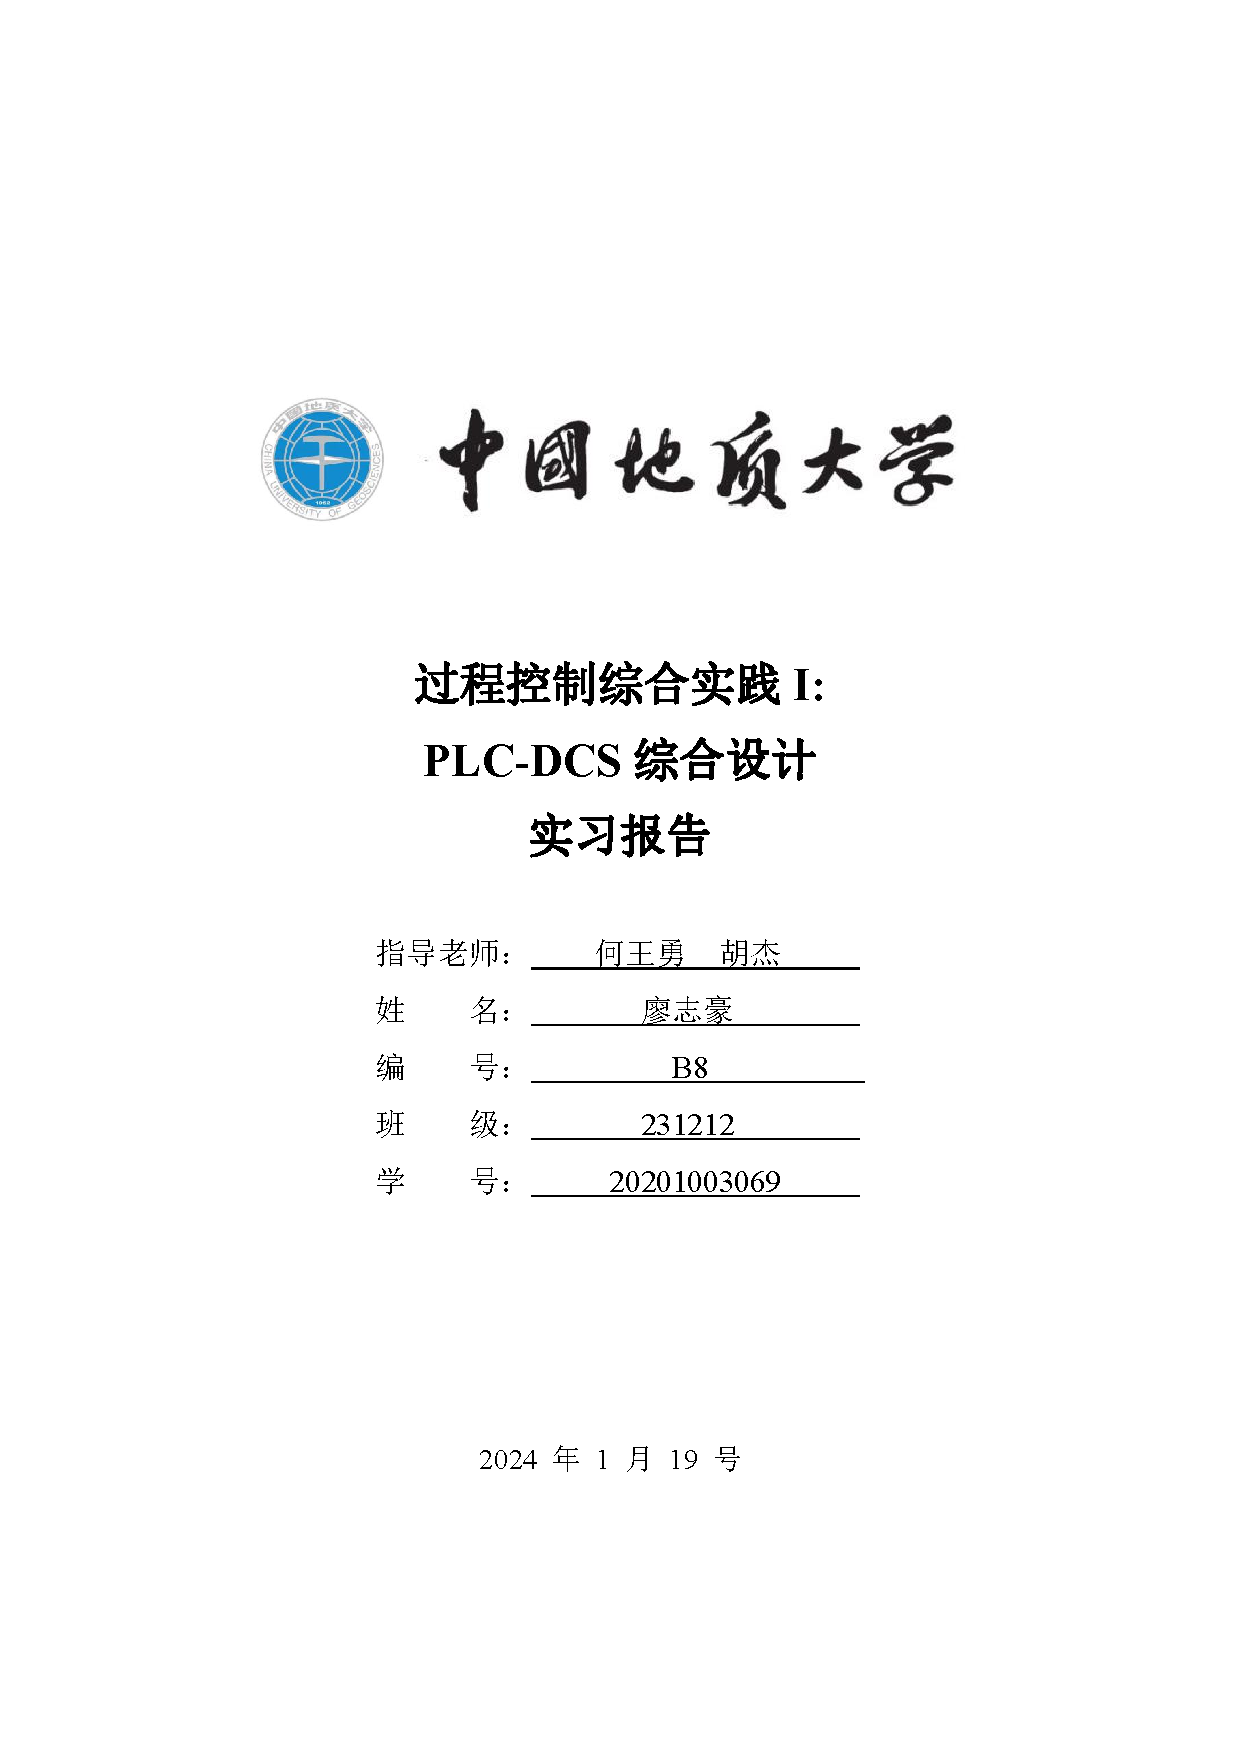
\includepdf[pages={1}]{cover.pdf}
% \end{titlepage}

% 生成目录
% \tableofcontents
% \cleardoublepage

% 导入图片
% \begin{figure}[H]
%     \centering % 居中 
%     % 图片文件的相对路径
%     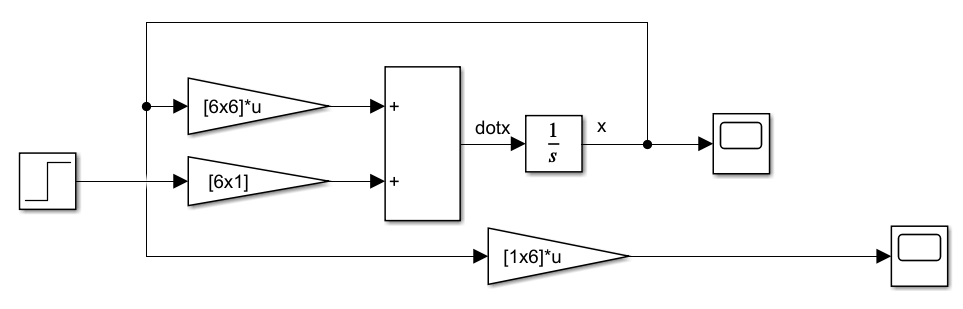
\includegraphics[width=.8\textwidth]{figure/exp1_1_model.png} 
%     \caption{Simulink模型} % caption是图片的标题
%     % \label{img} % 此处的label相当于一个图片的专属标志,目的是方便上下文的引用
% \end{figure}

% 导入代码
% \begin{lstlisting}
% a
% \end{lstlisting}



% \documentclass[twocolumn]{article}
\usepackage{flushend}
\usepackage{abstract}
\begin{document}
\title{基于直流减速电机输入电压和转角转速的系统参数辨识}
\author{作者:廖志豪 \quad 班级:231212 \quad 学号:20201003069}

% 摘要部分,不分栏
\twocolumn[
    \maketitle
    \begin{onecolabstract}
        直流减速电机(DC Reducer Motor)是一种广泛应用于工业领域的电动机,一般由直流电机和齿轮减速箱组成。其通常采用直流电作为输入,通过减速器将高速低扭矩转换为低速高扭矩的输出。本文采用基于递推最小二乘参数辨识、递推极大似然参数辨识和Newton-Raphson极大似然参数辨识等三种参数辨识方法,利用已有的数据集对典型直流电机进行基于差分方程模型的系统辨识。通过将模型输出与系统实际输出数据进行比较,均获得了较为理想的参数辨识结果。
    \end{onecolabstract}
]


% 请针对某一具体的需要进行参数辨识的实际系统,尝试使用本课程介绍的几种辨识方法(不少于两种),对系统参数进行辨识。
% 要求:
% 说明该实际系统的的研究意义;
% 给出所采用的几种辨识方法的原理及异同点;
% 给出辨识方法对应的算法、程序框图及代码(代码附后);
% 给出并分析辨识结果;
% 报告要符合发表论文的格式要求

%
\section{研究意义及研究对象介绍}
%%
\subsection{研究意义}
直流减速电机(DC Reducer Motor)是一种广泛应用于工业领域的电动机,其主要特点是在输入端接入直流电源,通过减速器将高速低扭矩转换为低速高扭矩的输出。直流减速电机在工业生产中具有重要的应用价值,如物流输送、自动化生产线、机器人关节等。因此,对直流减速电机的系统模型辨识具有重要的研究意义。

提高系统控制性能:通过对直流减速电机的模型辨识,可以建立其相对精确的数学模型,从而为控制系统设计提供依据。基于模型的控制策略(模型预测控制,MPC)可以提高系统的动态性能、稳态性能和抗干扰能力,实现对直流减速电机更精确的控制。

降低能耗:直流减速电机在运行过程中,其效率受到多种因素的影响,如负载变化、电源电压波动等。通过对直流减速电机的模型辨识,可以分析这些因素对电机效率的影响规律,从而制定相应的优化策略,降低能耗,提高能源利用率。

故障诊断与预测:直流减速电机在运行过程中可能出现各种故障,如轴承磨损、绕组短路等。通过对电机的模型辨识,可以建立故障特征参数与故障类型之间的对应关系,揭示出电机内部的一些异常情况,从而实现对电机故障的实时监测和预测,及时对电机进行检修维护或更换损坏部件,以提高设备的可靠性和安全性。

优化设计与制造:通过对直流减速电机的模型辨识,可以分析电机在不同工况下的运行特性,为电机的设计和制造提供参考。例如,可以根据模型辨识结果调整电机的结构参数、材料选择等,以提高电机的性能和使用寿命。

促进产业升级:直流减速电机在工业领域的广泛应用,对其性能和控制技术提出了更高的要求。通过对直流减速电机的模型辨识研究,可以为相关产业提供技术支持,推动产业升级,提高整体竞争力。

综上所述,基于直流减速电机模型辨识的研究对于提高电机系统控制性能、降低能耗、故障诊断与预测、优化设计与制造以及促进产业升级等方面具有重要的意义。





% 辨识得到的模型能够在一定程度上反映出直流减速电机的实际动态特性,从而有助于设计出更优的控制策略,进一步提升和优化系统的性能。

% 通过系统辨识得到的模型,可以用于预测在给定输入情况下直流减速电机的输出响应,为控制系统的设计和调试提供便利。

% 在模型参数辨识结果合理的前提下,通过对系统的输出理论值和实际值之间的比较,可以揭示出电机内部的一些异常情况,这对于实现故障诊断和预防性维护具有重要意义。

% %%%%%%%%%%%%%%%%%%%%%%%%%%%%%%%


% 首先,通过模型辨识,我们可以更准确地了解和把握直流减速电机的内部结构和运行机制。例如,可以获取到电机的电动势常数、转矩常数、自电感等关键参数,这些参数对于设计和优化控制器具有重要作用,有助于提高对直流减速电机的控制精度。此外,辨识出的模型能够反映直流减速电机的动态特性,从而有助于设计出更优的控制策略,进一步提升系统的性能。

% 其次,通过模型辨识,我们可以获得直流减速电机的数学模型。这个模型可以用来预测在给定输入情况下直流减速电机的输出响应,为控制系统的设计和调试提供便利。



%%
\subsection{直流减速电机简介}

直流减速电机,也称为齿轮减速电机,是在普通直流电机的基础上,加上配套齿轮减速箱而构成。这种配置的作用是提供较低的转速和较大的力矩,以满足各种工业应用的需求。

直流减速电机一般用于低转速大扭矩的传动设备,通过输入轴上的小齿轮与输出轴上的大齿轮啮合,达到降低转速、提高扭矩的目的。因此,直流减速电机是一个复杂的动力学系统,其阶次和动态性能取决于多种因素,包括电源电压、电流、负载等。这里以简单的直流电机为例,一个典型的直流电机的模型如下:
\begin{figure}[H]
    \centering % 居中 
    % 图片文件的相对路径
    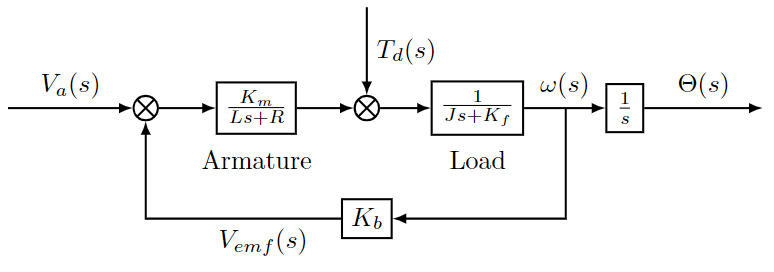
\includegraphics[width=.45\textwidth]{figure/直流电机模型.png} 
    \caption{典型直流电机模型} % caption是图片的标题
    % \label{img} % 此处的label相当于一个图片的专属标志,目的是方便上下文的引用
\end{figure}

其中$K_m$为力矩系数,$K_b$为反电势系数,$L$为线圈电感,$R$为线圈电阻,$J$为转子转动惯量,$K_f$为转子阻尼系数,$T_d$为负载,$\omega$为转子速度,$\theta$为转子位置,$V_a$为端部电压。此为理想直流电机的开环模型,其中的关键变量可以由以下方程得到:

\noindent 电压平衡方程:
\begin{equation*}
	V_a(t) = R_i(t) + L\frac{di(t)}{dt} + V_{emf}(t)
\end{equation*}
反电势方程:
\begin{equation*}
	V_{emf}(t) = K_b \dot{\theta}(t) = K_b \omega(t)
\end{equation*}
力矩方程:
\begin{equation*}
	T_a(t) = K_m \cdot i(t)
\end{equation*}
转子力矩平衡方程:
\begin{equation*}
	J \ddot{\theta}(t) = T_a(t) - T_d(t) - K_f\dot{\theta}(t)
\end{equation*}

由于$L$通常很小,而且电气时间常数一般远小于机械时间常数,此处我们可以忽略电感$L$。则根据以上条件可以得到直流电机的状态方程为:
\begin{equation*}
	\dot{x}(t) = 
	\begin{bmatrix}
		0 & 1 \\
		0 & -\frac{1}{\tau}
	\end{bmatrix} x(t) + 
	\begin{bmatrix}
		0 \\
		\frac{\beta}{\tau}
	\end{bmatrix} u(t) + 
	\begin{bmatrix}
		0 \\
		\frac{\gamma}{\tau}
	\end{bmatrix} T_d(t)
\end{equation*}
其中:
\begin{equation*}
	\begin{split}
		\tau = \frac{JR}{K_fR + K_mK_b} \\
		\beta = \frac{K_m}{K_fR + K_mK_b} \\
		\gamma = -\frac{R}{K_fR + K_mK_b}
	\end{split}
\end{equation*}
其中状态变量分别为电机转角和转速,即:
\begin{equation*}
	x(t) = 
	\begin{bmatrix}
		\theta(t) \\
		\dot{\theta}(t)
	\end{bmatrix} = 
	\begin{bmatrix}
		\theta(t) \\
		\omega(t)
	\end{bmatrix}
\end{equation*}
因此,按照通常的处理方法,我们可以将直流减速电机看做一个二阶系统,其差分方程模型为:
\begin{align*}
	y(k) &= -a_1y(k-1) - a_2u(k-2) + \\
	& b_1u(k-1) + b_2u(k-2) + v(k)
\end{align*}
其中$v(k)$为噪声项,此处我们假设该噪声项为常见的高斯白噪声,以便于进行接下来的系统参数辨识。

%
\section{辨识方法原理}
% 给出原理和异同点
%%
\subsection{递推最小二乘参数辨识方法}
递推最小二乘法采用参数递推估计,其大致思路为:
\begin{center}
    当前估计值$\hat{\theta}(k)$ = 上次估计值$\hat{\theta}(k+1)$ + 修正项
\end{center}

递推最小二乘算法的计算公式如下:
\begin{equation*}
    \hat{\theta}_{m+1} = \hat{\theta}_{m} + K_{m+1}[z(m+1) - h(m+1)\hat{\theta}_m]
\end{equation*}
\begin{align*}
    P_{m+1} &= P_m - P_m h^T(m+1) [w^{-1}(m+1) + h(m+1) \\
	& P_m h^T(m+1)]^{-1} h(m+1) P_m \\
    &= P_m - K_{m+1} K_{m+1}^T[w^{-1}(m+1) \\
	& + h(m+1) P_m h^T(m+1)]
\end{align*}
\begin{equation*}
    K_{m+1} = P_m h^T(m+1) [w^{-1}(m+1) + h(m+1) P_m h^T(m+1)]^{-1}
\end{equation*}
对部分变量解释如下:
\begin{itemize}
    \item $\hat{\theta}_m$:前一时刻的参数估值
    \item $z(m+1)$:当前时刻的量测值
    \item $h(m+1) \hat{\theta}_m$:在前一量测的基础上对在$(m+1)$的预测
    \item $z(m+1) - h(m+1) \hat{\theta}_m$:预测误差,又称为新息
    \item $K_{m+1}$:修正的增益矩阵
\end{itemize}

此外,关于递归参数估计的停止条件,可以指定迭代的次数,也可以指定相邻两次参数估计值的偏差大小$\varepsilon$:
\begin{equation*}
    \forall{i} \ \max | \frac{\hat{\theta}_i(m+1) - \hat{\theta}_i(m)}{\hat{\theta}_i(m)} | < \varepsilon
\end{equation*}

%%
\subsection{递推极大似然参数辨识方法}
设离散随机过程${Y_k}$与未知参数$\theta$有关,假定已知概率分布密度函数$f(Y_k|\theta)$。如果我们得到$n$个独立的观测值:$Y_1,\ Y_2,\ …,\ Y_n$,则可得概率密度分布分别为:$f(Y_1|\theta),\ f(Y_2|\theta),\ …,$ $\ f(Y_n|\theta)$。要求根据这些观测值来估计未知参数$\theta$,估计的准则是使得观测值${Y_k}$的出现概率为最大。为此,定义一个似然函数:
\begin{equation*}
    L(Y_1,\ Y_2,\ \dots,\ Y_N|\theta) = f(Y_1|\theta)f(Y_2|\theta)\dots(Y_N|\theta)
\end{equation*}

上式的右边是$n$个概率密度函数的连乘,似然函数$L$是$\theta$的函数。如果$L$达到最大值,则${Y_k}$出现的概率为最大。因此极大似然法的实质就是求出使得$L$达到极大值的$\theta$的估值。对上式取对数并求偏导即可得到$\theta$的极大似然估计:
\begin{equation*}
    \hat{\theta}_{ML} = \frac{1}{N}\sum_{i=1}^Ny_i
\end{equation*}

极大似然法辨识的物理意义:根据一组确定的随机序列$Y_N$,设法找到参数估计值$\hat{\theta}_{ML}$,它使得随机变量$y$在$\hat{\theta}_{ML}$条件下的概率密度函数最大可能地逼近随机变量$y$在$\theta$(真值)条件下的概率密度函数,即:
\begin{equation*}
    p(y|\hat{\theta}_{ML}) \stackrel{max}{--\rightarrow} p(y|\theta)
\end{equation*}

%%
\subsection{Newton-Raphson方法原理}
\paragraph{Newton-Raphson方法的思想}~{}

根据第L次迭代得到的参数估计$\hat{\theta}(L),\ \hat{\theta}(L + 1)$:
\begin{equation*}
    J_{L + 1}(\hat{\theta}(L + 1)) \le J_L(\hat{\theta}(L)) 
\end{equation*}
其中:
\begin{equation*}
    J_L(\theta) = \frac{1}{2}\sum_{k = (L - 1)N + n + 1}^{NL + n}\varepsilon^2(k) 
\end{equation*}


\paragraph{Newton-Raphson法应用于极大似然参数估计}~{}

Newton-Raphson法应用于极大似然估计求解的步骤:
\begin{enumerate}
    \item 确定初始值$\hat{\theta}_0$
    
    先采集一批输入输出数据$\{ y(k) \},\ \{ u(k) \}$,用最小二乘法获得$\hat{a}_1, ..., \hat{a}_n,$ $\hat{b}_1, ..., \hat{b}_n$,对于$\hat{\theta}(L)$中的$\hat{d}_1, ..., \hat{d}_n$,可先任意假定初值。

    \item 设定初始参数值
    \begin{equation*}
		\varepsilon(1), \varepsilon(2), ..., \varepsilon(n)
	\end{equation*} 
	\begin{equation*}
		\frac{\partial\varepsilon(1)}{\partial\theta}|_{\theta = \hat{\theta}(L)},\frac{\partial\varepsilon(2)}{\partial\theta}|_{\theta = \hat{\theta}(L)}, ..., \frac{\partial\varepsilon(n)}{\partial\theta}|_{\theta = \hat{\theta}(L)}
	\end{equation*} 
	为方便起见,通常均取零。
    
    \item 计算$\varepsilon(k)$
    
    采集一批长度为N的数据$\{ y(k) \}, \{ u(k) \}$,利用$\hat{\theta}(L)$和$\varepsilon(k)$,根据下式计算新的$\varepsilon(k)(k = NL + n + 1, NL + n + 2, ..., NL + n + N)$:
	\begin{align*}
		\varepsilon(k) &= y(k) + \sum_{i = 1}^n \hat{a}_iy(k - i) \\
		& - \sum_{i = 1}^n \hat{b}_iu(k - i) - \sum_{i = 1}^n \hat{d}_i\varepsilon(k - i) \\
	\end{align*}

    \item 计算$\frac{\partial \varepsilon(k)}{\partial \theta}|_{\theta = \hat{\theta}(L)}(k = NL + n + 1, NL + n + 2, ..., NL + n + N)$
    
    根据下式计算$\frac{\partial \varepsilon(k)}{\partial \theta}|_{\theta = \hat{\theta}(L)}$:
    \begin{equation*}
        \frac{\partial\varepsilon(k)}{\partial a_j} = y(k - j) - \sum_{i = 1}^n d_i \frac{\partial \varepsilon(k - i)}{\partial a_j}|_{\theta = \hat{\theta}(L)} 
    \end{equation*}
    \begin{equation*}
        \frac{\partial \varepsilon(k)}{\partial b_j} = -u(k - j) - \sum_{i = 1}^n d_i \frac{\partial \varepsilon(k - i)}{\partial b_j}|_{\theta = \hat{\theta}(L)}
    \end{equation*}
    \begin{equation*}
        \frac{\partial \varepsilon(k)}{\partial d_j} = -\varepsilon(k - j) - \sum_{i = 1}^n d_i \frac{\partial \varepsilon(k - i)}{\partial d_j}|_{\theta = \hat{\theta}(L)}
    \end{equation*}

    \item 计算梯度阵和$Hessian$阵
	% 计算梯度阵$\frac{\partial J_{L + 1}}{\partial \theta}|_{\theta = \hat{\theta}(L)}$和$Hessian$阵$\frac{\partial^2 J_{L + 1}}{\partial (\theta)^2}|_{\theta = \hat{\theta}(L)}$
    
    利用所计算的$\varepsilon(k)$和$\frac{\partial \varepsilon(k)}{\partial \theta}|_{\theta = \hat{\theta}(L)}$:
    \begin{equation*}
        \frac{\partial J_{L + 1}}{\partial \theta}|_{\theta = \hat{\theta}(L)} = \sum_{k = NL + n + 1}^{(L + 1)N + n} \varepsilon(k) \cdot \frac{\partial \varepsilon(k)}{\partial \theta}|_{\theta = \hat{\theta}(L)} 
    \end{equation*}
    \begin{equation*}
        \frac{\partial^2 J_{L + 1}}{\partial (\theta)^2}|_{\theta = \hat{\theta}(L)} \approx \sum_{k = NL + n + 1}^{(L + 1)N + n}\frac{\partial \varepsilon(k)}{\partial \theta}[\frac{\partial \varepsilon(k)}{\partial \theta}]^T|_{\theta = \hat{\theta}(L)}
    \end{equation*}

    \item 计算新的估值$\hat{\theta}(L + 1)$
    \begin{equation*}
        \hat{\theta}(L + 1) = \hat{\theta}(L) - [\frac{\partial^2 J_{L + 1}}{\partial (\theta)^2}]^{-1}|_{\theta = \hat{\theta}(L)} \cdot \frac{\partial J_{L + 1}}{\partial \theta}|_{\theta = \hat{\theta}(L)}
    \end{equation*}

    \item 取最后$n$个$\varepsilon(k)$和$\frac{\partial \varepsilon(k)}{\partial \theta}_{\theta = \hat{\theta}(L)}$值,作为下一次迭代的初值,$L = L + 1$,转到 $3.$ 继续循环,直至满足停止条件。设经过$r$次迭代计算后得到$\hat{\theta}(r)$,则停止迭代标准为:
    \begin{equation*}
        || \hat{\theta}(r + 1) - \hat{\theta}(r) || \le \Delta 
    \end{equation*}
    \begin{equation*}
        | \frac{\sigma_{r + 1}^2 - \sigma_r^2}{\sigma_r^2} | \le \nu, \quad r = M
    \end{equation*}
\end{enumerate}

\paragraph{说明}~{}
\begin{enumerate}
    \item 该数值算法即使当系统噪声水平较高时也能获得良好的估计
    \item 需要进行N次观测,才能进行一次递推
\end{enumerate}

%%
\subsection{异同点分析}
递推最小二乘参数辨识、递推极大似然参数辨识和Newton-Raphson极大似然参数辨识都是用于系统模型参数估计的方法。它们的主要区别在于所采用的优化准则不同,因此导致这些算法在程序实现方面和参数辨识性能上也存在一些差异。

递推最小二乘参数辨识方法:该方法基于最小二乘法原理,通过迭代计算来估计系统模型的参数。其基本思想是将观测数据与模型输出之间的误差平方和最小化作为优化目标,然后利用梯度下降等优化算法进行求解。该方法具有简单、快速、收敛性好等优点,但需要对系统模型的非线性程度进行限制,否则可能导致局部最优解的问题。

递推极大似然参数辨识方法:该方法基于极大似然估计原理,通过迭代计算来估计系统模型的参数。其基本思想是将观测数据与模型输出之间的似然函数最大化作为优化目标,之后可以利用优化算法进行求解。该方法具有精度高、鲁棒性强等优点,但需要对系统模型的线性程度进行限制,否则可能导致不收敛的问题。

Newton-Raphson极大似然参数辨识方法:该方法是递推极大似然参数辨识方法的一种改进形式,它采用了牛顿-拉夫逊迭代法来求解优化问题。相比于传统的递推极大似然参数辨识方法,该方法具有更快的收敛速度和更高的精度。但是,由于牛顿-拉夫逊迭代法需要计算Hessian矩阵,因此计算复杂度较高,且容易陷入局部最优解的问题。

综上所述,三种方法各有优缺点,具体选择哪种方法取决于实际应用场景和需求。如果要求快速收敛和简单实现,可以选择递推最小二乘参数辨识方法;如果要求高精度和鲁棒性,可以选择递推极大似然参数辨识方法或Newton-Raphson极大似然参数辨识方法;如果要求更高的精度和更快的收敛速度,则可以选择Newton-Raphson极大似然参数辨识方法。

%
\section{算法及程序框图}
本次直流电机系统参数辨识采用matlab软件提供的数据集dcmdata,数据集内包含包含一组输入数据(输入电压)和两组输出数据(电机转角和转速),每组数据共400个采样点,采样周期为0.1s,如下图所示:
\begin{figure}[H]
    \centering % 居中 
    % 图片文件的相对路径
    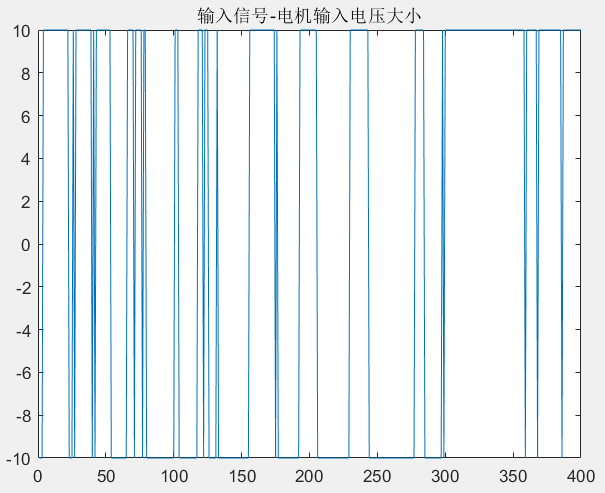
\includegraphics[width=.4\textwidth]{figure/输入信号-电机输入电压大小.png} 
    \caption{输入信号-电机输入电压大小} % caption是图片的标题
    % \label{img} % 此处的label相当于一个图片的专属标志,目的是方便上下文的引用
\end{figure}
\begin{figure}[H]
    \centering % 居中 
    % 图片文件的相对路径
    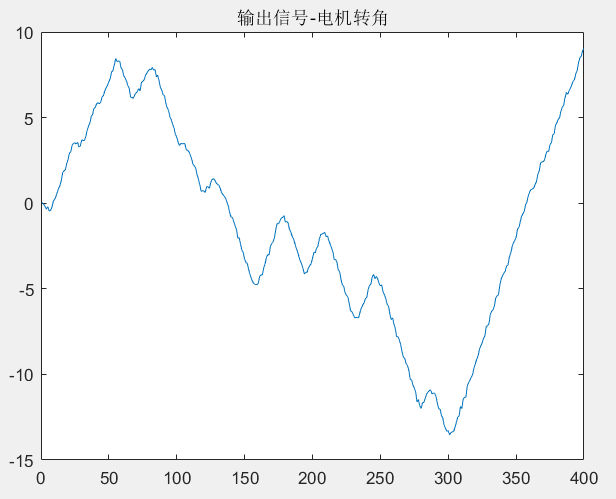
\includegraphics[width=.4\textwidth]{figure/输出信号-电机转角.png} 
    \caption{输出信号-电机转角} % caption是图片的标题
    % \label{img} % 此处的label相当于一个图片的专属标志,目的是方便上下文的引用
\end{figure}

由图可以看出,输入信号为类似于M序列的随机等幅波动信号,两组输出信号中,电机转角信号受噪声影响较小,而电机转速信号受噪声影响较大,在波峰波谷处存在明显的抖动。

\begin{figure}[H]
    \centering % 居中 
    % 图片文件的相对路径
    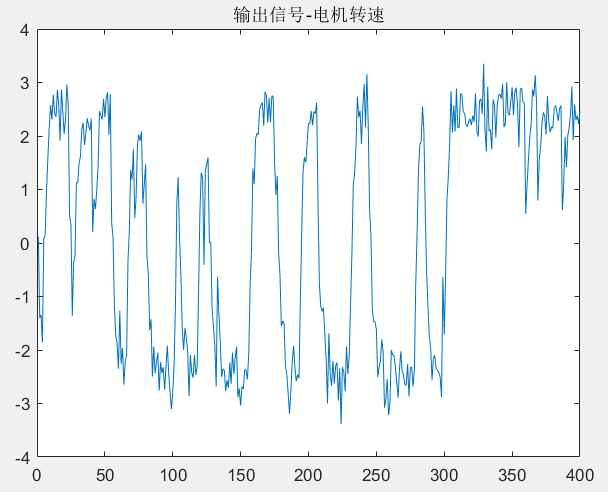
\includegraphics[width=.4\textwidth]{figure/输出信号-电机转速.png} 
    \caption{输出信号-电机转速} % caption是图片的标题
    % \label{img} % 此处的label相当于一个图片的专属标志,目的是方便上下文的引用
\end{figure}

此处假设观测数据中的噪声为高斯白噪声,且考虑到我们采用的参数辨识算法对于噪声项参数具有一定的辨识能力,此处对原始数据不额外采用滤波处理。下面分别针对输入电压-电机转角和输入电压-电机转速进行系统参数辨识。

%%
\subsection{递推最小二乘参数辨识方法}
\paragraph{程序框图}~{}
% 递推最小二乘参数辨识 直流电机
\begin{figure}[H]
    \centering % 居中 
    % 图片文件的相对路径
    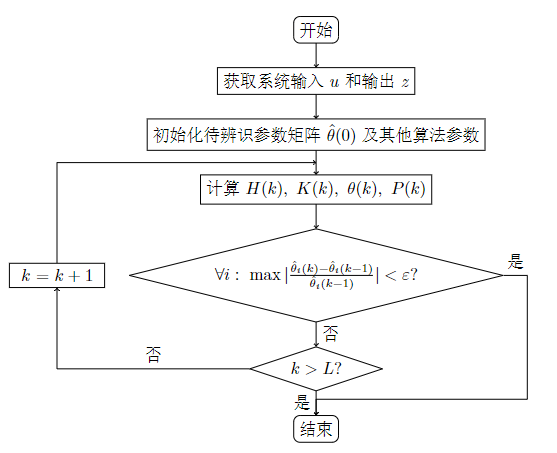
\includegraphics[width=0.45\textwidth]{figure/最小二乘-程序框图.png} 
    \caption{递推最小二乘参数辨识-程序框图} % caption是图片的标题
    % \label{img} % 此处的label相当于一个图片的专属标志,目的是方便上下文的引用
\end{figure}

%%
\subsection{递推极大似然参数辨识方法}
\paragraph{程序框图}~{}
% 递推极大似然参数辨识 直流电机
\begin{figure}[H]
    \centering % 居中 
    % 图片文件的相对路径
    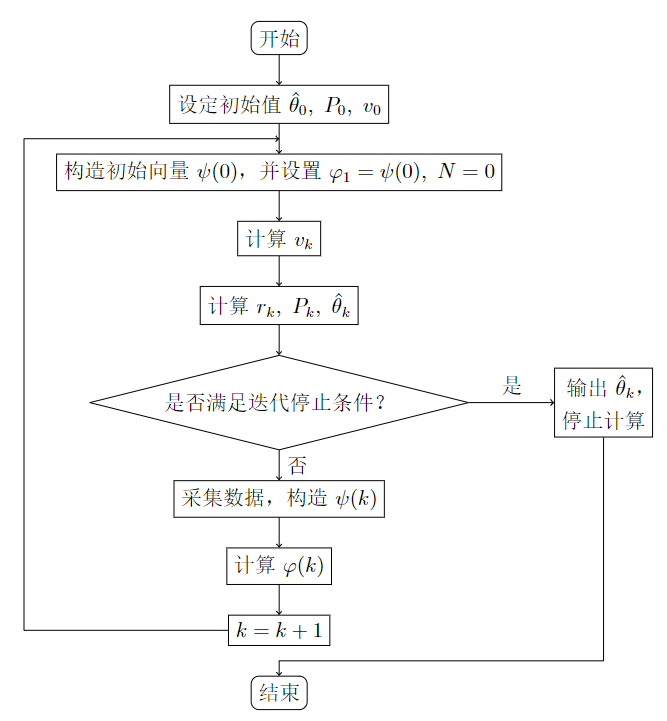
\includegraphics[width=.45\textwidth]{figure/极大似然-程序框图.png} 
    \caption{递推极大似然参数辨识方法-程序框图} % caption是图片的标题
    % \label{img} % 此处的label相当于一个图片的专属标志,目的是方便上下文的引用
\end{figure}

%%
\subsection{Newton-Raphson极大似然参数辨识方法}
\paragraph{程序框图}~{}
% Newton-Raphson方法 电机辨识
\begin{figure}[H]
    \centering % 居中 
    % 图片文件的相对路径
    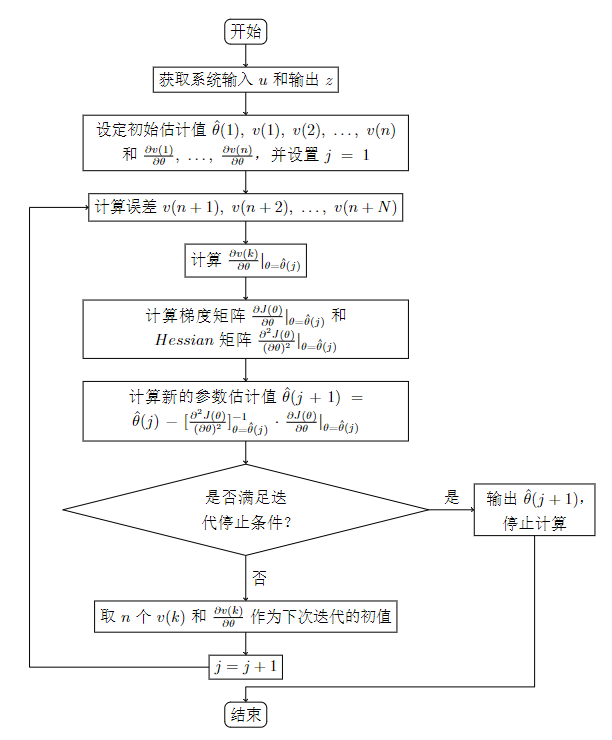
\includegraphics[width=.45\textwidth]{figure/newton-程序框图.png} 
    \caption{Newton-Raphson方法参数估计-程序框图} % caption是图片的标题
    % \label{img} % 此处的label相当于一个图片的专属标志,目的是方便上下文的引用
\end{figure}

%
\section{辨识结果及分析}

%%
\subsection{递推最小二乘参数辨识方法}
%%%
\paragraph{输入电压-电机转角}~{}

迭代400次以后,最终的参数辨识结果如下:
\begin{table}[H] % 防止表格乱跑
\centering % 居中
\begin{tabular}{cc} % 指明列数
	\toprule % 顶部粗线
	辨识参数 & 辨识结果 \\
	\midrule % 中间细线
	$a_1$ & -0.9385 \\
	$a_2$ & -0.0632 \\
	$b_1$ & 0.0072 \\
	$b_2$ & 0.0147 \\
	\bottomrule % 底部粗线
\end{tabular}
\caption{参数辨识结果:输入电压-电机转角} % 标题
\end{table}

系统实际输出与经过参数辨识后得到的模型输出比较如下:
\begin{figure}[H]
    \centering % 居中 
    % 图片文件的相对路径
    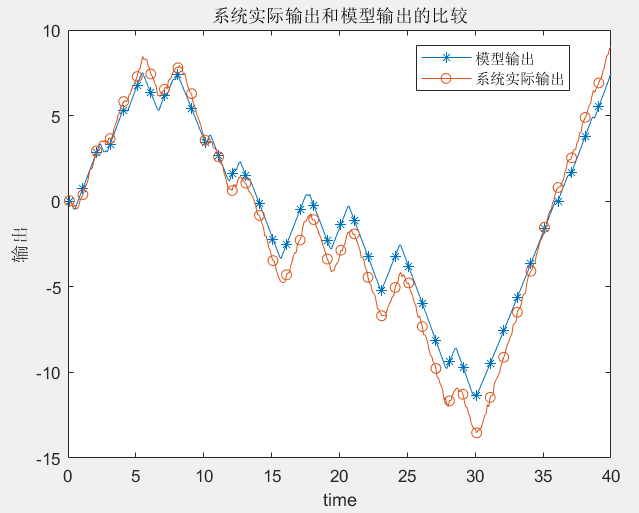
\includegraphics[width=.4\textwidth]{figure/最小二乘-电机转角-输出比较.png} 
    \caption{输出信号比较} % caption是图片的标题
    % \label{img} % 此处的label相当于一个图片的专属标志,目的是方便上下文的引用
\end{figure}
由于无法准确得知获取系统输出观测数据时的噪声情况,此处在获取模型输出时均未考虑噪声项部分的影响。可以看到,模型输出与系统实际输出之间基本一致,说明参数辨识效果较好。

迭代过程中的参数辨识情况如下:
\begin{figure}[H]
    \centering % 居中 
    % 图片文件的相对路径
    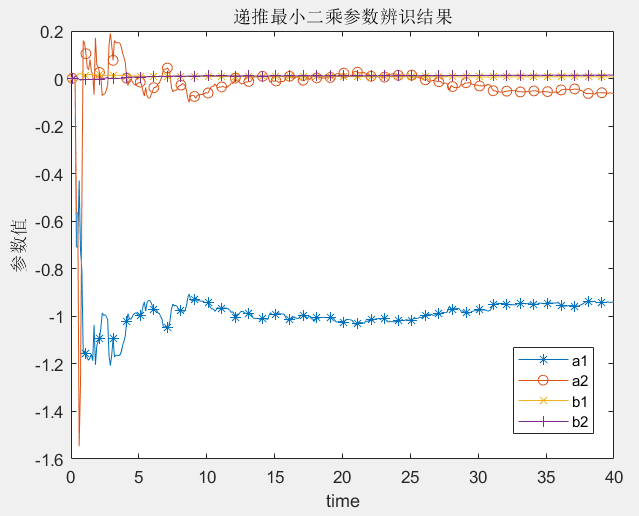
\includegraphics[width=.4\textwidth]{figure/最小二乘-电机转角-参数辨识结果.png} 
    \caption{参数辨识结果} % caption是图片的标题
    % \label{img} % 此处的label相当于一个图片的专属标志,目的是方便上下文的引用
\end{figure}

参数辨识精度的变化情况如下,此处将参数辨识精度值取为相邻两次参数辨识值之间的差值:
\begin{figure}[H]
    \centering % 居中 
    % 图片文件的相对路径
    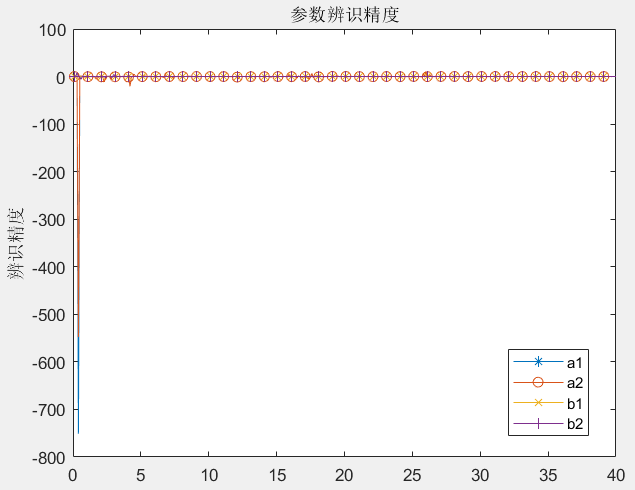
\includegraphics[width=.4\textwidth]{figure/最小二乘-电机转角-参数辨识精度.png} 
    \caption{参数辨识精度} % caption是图片的标题
    % \label{img} % 此处的label相当于一个图片的专属标志,目的是方便上下文的引用
\end{figure}
根据以上参数辨识的收敛情况以及参数辨识精度变化情况可以发现,各参数在经过约100次迭代以后已基本趋于稳定,且辨识精度基本维持在较高水平,表明了递推最小二乘参数辨识方法收敛速度快的特点。

%%%
\paragraph{输入电压-电机转速}~{}

在经过400次迭代以后,最终的参数辨识结果如下:
\begin{table}[H] % 防止表格乱跑
\centering % 居中
\begin{tabular}{cc} % 指明列数
	\toprule % 顶部粗线
	辨识参数 & 辨识结果 \\
	\midrule % 中间细线
	$a_1$ & -0.2000 \\
	$a_2$ & -0.2919 \\
	$b_1$ & 0.0864 \\
	$b_2$ & 0.0387 \\
	\bottomrule % 底部粗线
\end{tabular}
\caption{参数辨识结果:输入电压-电机转速} % 标题
\end{table}

系统实际输出与经过参数辨识后得到的模型输出比较如下:
\begin{figure}[H]
    \centering % 居中 
    % 图片文件的相对路径
    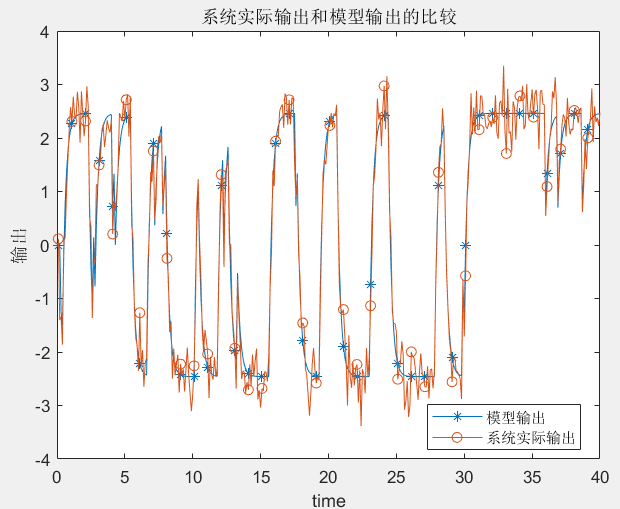
\includegraphics[width=.4\textwidth]{figure/最小二乘-电机转速-输出比较.png} 
    \caption{输出信号比较} % caption是图片的标题
    % \label{img} % 此处的label相当于一个图片的专属标志,目的是方便上下文的引用
\end{figure}

迭代过程中的参数辨识情况如下:
\begin{figure}[H]
    \centering % 居中 
    % 图片文件的相对路径
    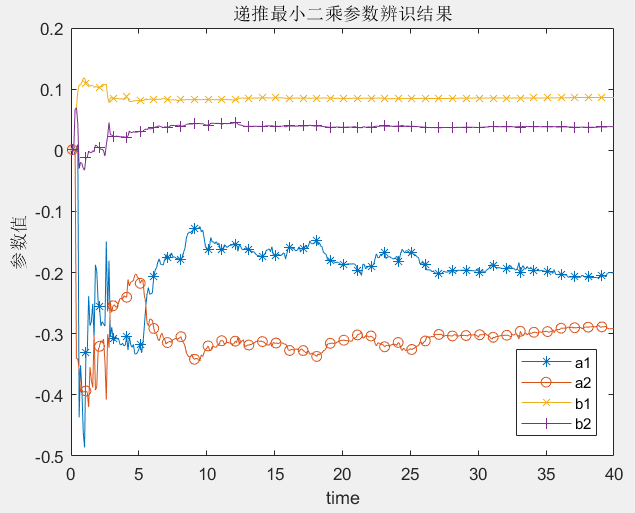
\includegraphics[width=.4\textwidth]{figure/最小二乘-电机转速-参数辨识结果.png} 
    \caption{参数辨识结果} % caption是图片的标题
    % \label{img} % 此处的label相当于一个图片的专属标志,目的是方便上下文的引用
\end{figure}

参数辨识精度的变化情况如下:
\begin{figure}[H]
    \centering % 居中 
    % 图片文件的相对路径
    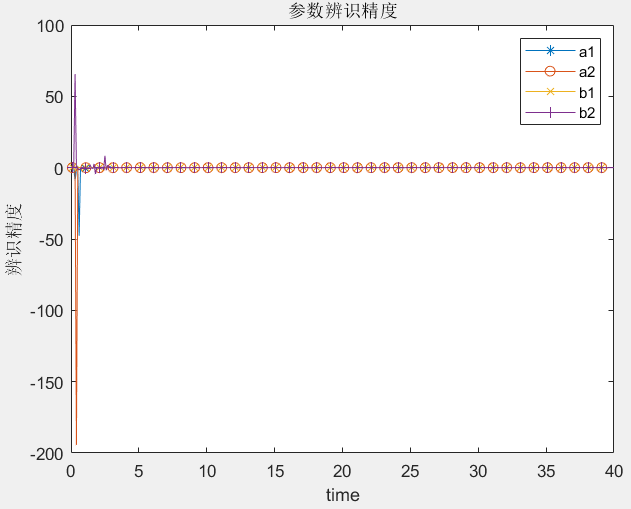
\includegraphics[width=.4\textwidth]{figure/最小二乘-电机转速-参数辨识精度.png} 
    \caption{参数辨识精度} % caption是图片的标题
    % \label{img} % 此处的label相当于一个图片的专属标志,目的是方便上下文的引用
\end{figure}


%%
\subsection{极大似然参数辨识方法}
%%%
\paragraph{输入电压-电机转角}~{}

最终的参数辨识结果如下:
\begin{table}[H] % 防止表格乱跑
\centering % 居中
\begin{tabular}{cc} % 指明列数
	\toprule % 顶部粗线
	辨识参数 & 辨识结果 \\
	\midrule % 中间细线
	$a_1$ & -0.9030 \\
	$a_2$ & -0.0986 \\
	$b_1$ &  0.0081	\\
	$b_2$ & 0.0144 \\
	$c_1$ & -0.0488 \\
    $c_2$ & 0.0606 \\
	\bottomrule % 底部粗线
\end{tabular}
\caption{参数辨识结果:输入电压-电机转角} % 标题
\end{table}

系统实际输出与经过参数辨识后得到的模型输出比较如下:
\begin{figure}[H]
    \centering % 居中 
    % 图片文件的相对路径
    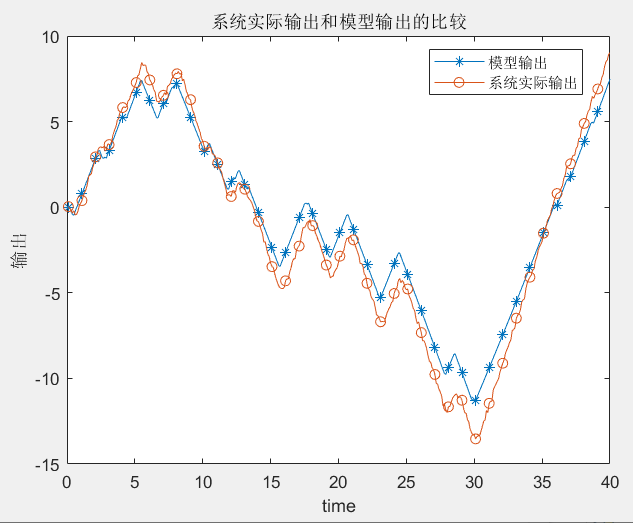
\includegraphics[width=.4\textwidth]{figure/极大似然-电机转角-输出比较.png} 
    \caption{输出信号比较} % caption是图片的标题
    % \label{img} % 此处的label相当于一个图片的专属标志,目的是方便上下文的引用
\end{figure}

迭代过程中的参数辨识情况如下:
\begin{figure}[H]
    \centering % 居中 
    % 图片文件的相对路径
    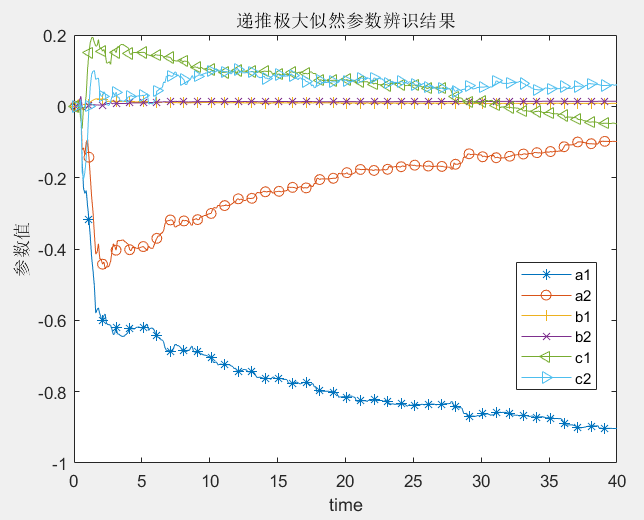
\includegraphics[width=.4\textwidth]{figure/极大似然-电机转角-参数辨识结果.png} 
    \caption{参数辨识结果} % caption是图片的标题
    % \label{img} % 此处的label相当于一个图片的专属标志,目的是方便上下文的引用
\end{figure}

参数辨识精度的变化情况如下:
\begin{figure}[H]
    \centering % 居中 
    % 图片文件的相对路径
    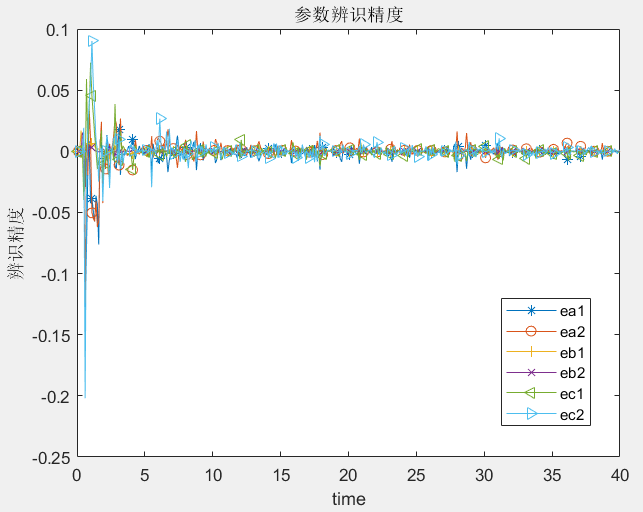
\includegraphics[width=.4\textwidth]{figure/极大似然-电机转角-参数辨识精度.png} 
    \caption{参数辨识精度} % caption是图片的标题
    % \label{img} % 此处的label相当于一个图片的专属标志,目的是方便上下文的引用
\end{figure}

%%%
\paragraph{输入电压-电机转速}~{}

最终的参数辨识结果如下:
\begin{table}[H] % 防止表格乱跑
\centering % 居中
\begin{tabular}{cc} % 指明列数
	\toprule % 顶部粗线
	辨识参数 & 辨识结果 \\
	\midrule % 中间细线
	$a_1$ & -0.1591 \\
	$a_2$ & -0.3340 \\
	$b_1$ & 0.0855 \\
	$b_2$ & 0.0409 \\
	$c_1$ & -0.1067 \\
    $c_2$ & -0.3401 \\
	\bottomrule % 底部粗线
\end{tabular}
\caption{参数辨识结果:输入电压-电机转速} % 标题
\end{table}

系统实际输出与经过参数辨识后得到的模型输出比较如下:
\begin{figure}[H]
    \centering % 居中 
    % 图片文件的相对路径
    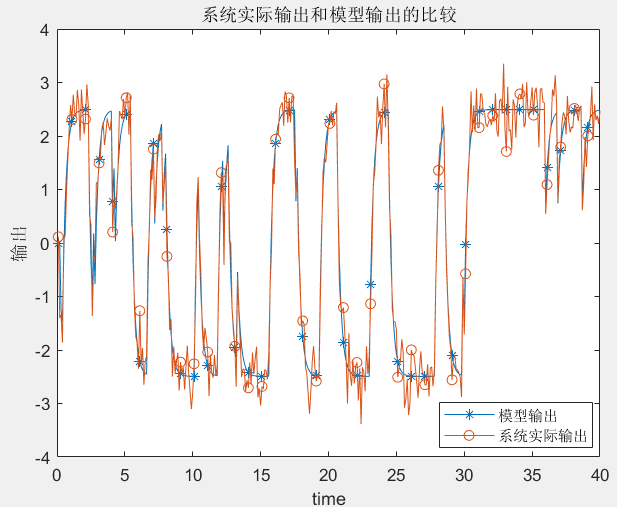
\includegraphics[width=.4\textwidth]{figure/极大似然-电机转速-输出比较.png} 
    \caption{输出信号比较} % caption是图片的标题
    % \label{img} % 此处的label相当于一个图片的专属标志,目的是方便上下文的引用
\end{figure}

迭代过程中的参数辨识情况如下:
\begin{figure}[H]
    \centering % 居中 
    % 图片文件的相对路径
    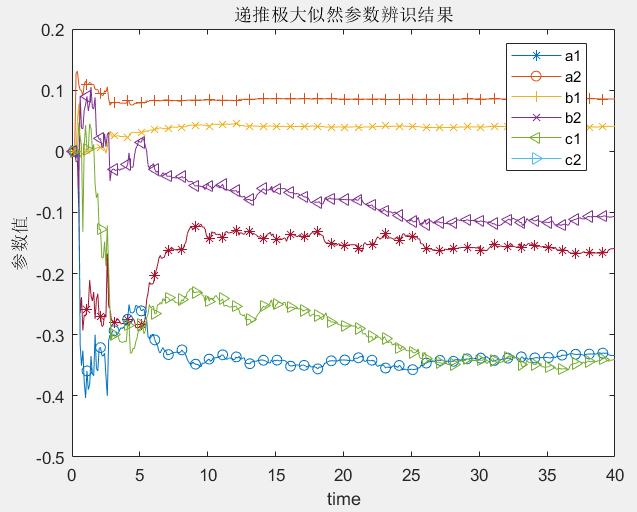
\includegraphics[width=.4\textwidth]{figure/极大似然-电机转速-参数辨识结果.png} 
    \caption{参数辨识结果} % caption是图片的标题
    % \label{img} % 此处的label相当于一个图片的专属标志,目的是方便上下文的引用
\end{figure}

参数辨识精度的变化情况如下:
\begin{figure}[H]
    \centering % 居中 
    % 图片文件的相对路径
    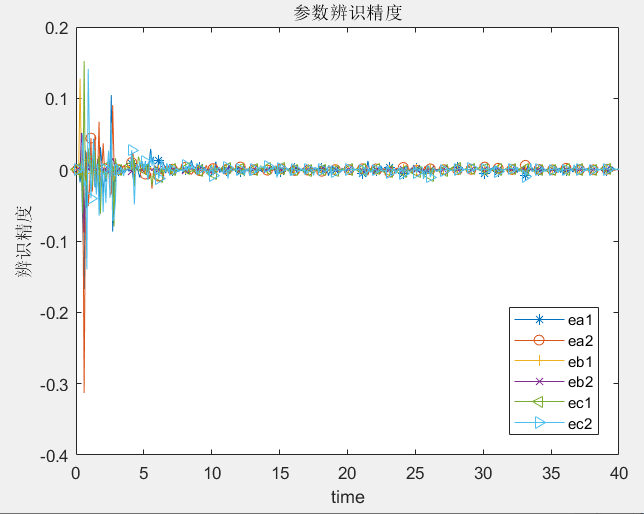
\includegraphics[width=.4\textwidth]{figure/极大似然-电机转速-参数辨识精度.png} 
    \caption{参数辨识精度} % caption是图片的标题
    % \label{img} % 此处的label相当于一个图片的专属标志,目的是方便上下文的引用
\end{figure}

由以上实验结果可以看出,极大似然参数估计递推算法在针对基于直流电机的输入电压-电机转角和输入电压-电机转速两组数据的系统参数辨识上具有和递推最小二乘参数辨识方法相似的表现。相比递推最小二乘参数辨识,递推极大似然参数辨识方法还可以对电机系统的噪声项参数进行辨识和估计,且整体上看具有相对较高的参数辨识精度。但是,递推极大似然参数辨识方法的参数收敛速度相对较慢,且计算量更大,因此在速度上相比基于最小二乘的参数辨识方法较慢。

%%
\subsection{Newton-Raphson极大似然参数辨识方法}
%%%
\paragraph{输入电压-电机转角}~{}

经过$2 \times 10^6$次迭代以后,最终的参数辨识结果如下:
\begin{table}[H] % 防止表格乱跑
\centering % 居中
\begin{tabular}{cc} % 指明列数
	\toprule % 顶部粗线
	辨识参数 & 辨识结果 \\
	\midrule % 中间细线
	$a_1$ & -1.5821 \\
	$a_2$ & 0.5821 \\
	$b_1$ & 0.0010 \\
	$b_2$ & 0.0093 \\
	$c_1$ & -1.0423 \\
	$c_2$ & 0.0564 \\
	\bottomrule % 底部粗线
\end{tabular}
\caption{参数辨识结果:输入电压-电机转角} % 标题
\end{table}

系统实际输出与经过参数辨识后得到的模型输出比较如下:
\begin{figure}[H]
    \centering % 居中 
    % 图片文件的相对路径
    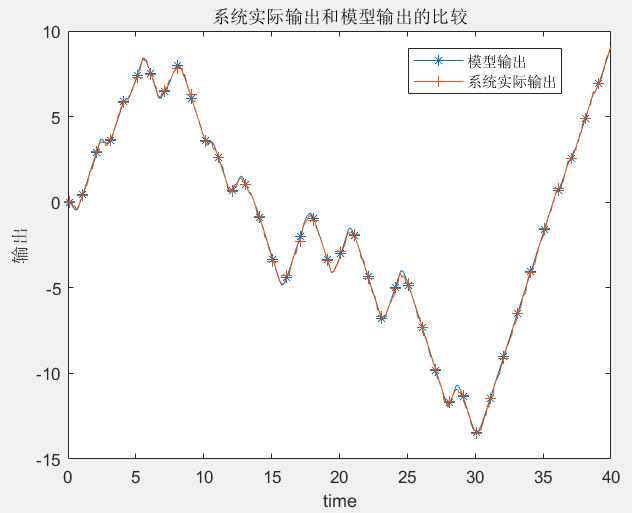
\includegraphics[width=.4\textwidth]{figure/newton-输出比较.png} 
    \caption{输出信号比较} % caption是图片的标题
    % \label{img} % 此处的label相当于一个图片的专属标志,目的是方便上下文的引用
\end{figure}
根据上图,模型输出与系统实际输出之间基本重合,说明Newton-Raphson极大似然参数辨识方法在经过充分迭代的情况下,其模型参数辨识的结果是较为理想的,其准确度明显高于其他两种方法。

迭代过程中的参数辨识情况如下:
\begin{figure}[H]
    \centering % 居中 
    % 图片文件的相对路径
    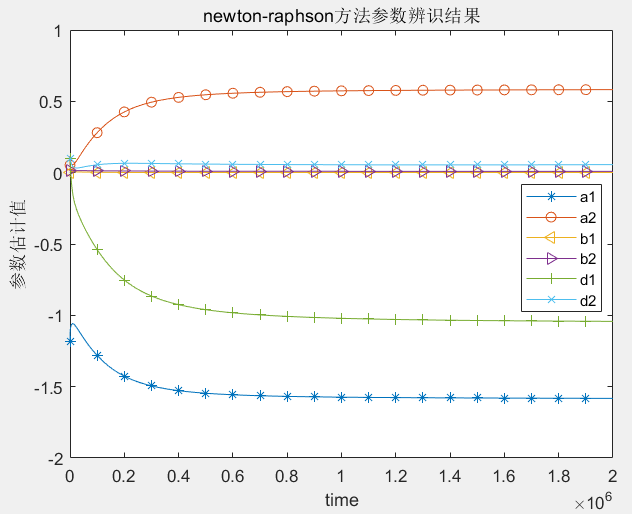
\includegraphics[width=.4\textwidth]{figure/newton-参数辨识结果.png} 
    \caption{参数辨识结果} % caption是图片的标题
    % \label{img} % 此处的label相当于一个图片的专属标志,目的是方便上下文的引用
\end{figure}

%%%
\paragraph{输入电压-电机转速}~{}

经过$2 \times 10^6$次迭代以后,最终的参数辨识结果如下:
\begin{table}[H] % 防止表格乱跑
\centering % 居中
\begin{tabular}{cc} % 指明列数
	\toprule % 顶部粗线
	辨识参数 & 辨识结果 \\
	\midrule % 中间细线
	$a_1$ & 0.0983 \\
	$a_2$ & -0.5024 \\
	$b_1$ & 0.0857 \\
	$b_2$ & 0.0629 \\
	$c_1$ & 0.1456 \\
	$c_2$ & -0.6023 \\
	\bottomrule % 底部粗线
\end{tabular}
\caption{参数辨识结果:输入电压-电机转速} % 标题
\end{table}

系统实际输出与经过参数辨识后得到的模型输出比较如下:
\begin{figure}[H]
    \centering % 居中 
    % 图片文件的相对路径
    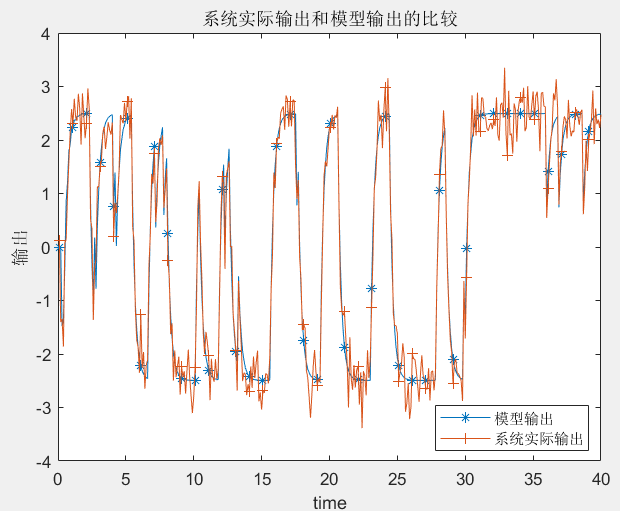
\includegraphics[width=.4\textwidth]{figure/newton-转速-输出比较.png} 
    \caption{输出信号比较} % caption是图片的标题
    % \label{img} % 此处的label相当于一个图片的专属标志,目的是方便上下文的引用
\end{figure}
此处获取模型输出时没有考虑噪声项部分对系统输出的影响,因此模型的输出比系统实际输出更稳定,减少了许多杂波。参照前面针对输入电压-电机转角的参数辨识结果可以知道,由于电机转角相对电机转速受到噪声干扰的影响更小,因此在进行输入电压-电机转角的参数辨识时,获得的模型输出与系统实际输出有着更高的重合度。

这里对比系统的实际输出以及模型的输出之间的差异可以看到,我们通过Newton-Raphson极大似然参数辨识方法最终获得的模型参数使得我们的模型输出特性和实际电机系统基本一致,仅在系统实际输出出现了较为严重的噪声波动时有较大偏差。

迭代过程中的参数辨识情况如下:
\begin{figure}[H]
    \centering % 居中 
    % 图片文件的相对路径
    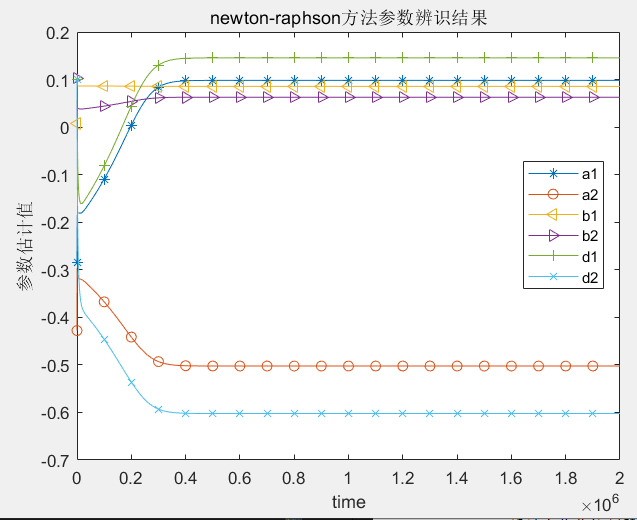
\includegraphics[width=.4\textwidth]{figure/newton-转速-辨识结果.png} 
    \caption{参数辨识结果} % caption是图片的标题
    % \label{img} % 此处的label相当于一个图片的专属标志,目的是方便上下文的引用
\end{figure}
根据各参数辨识值的收敛情况可以清楚地看到,所有模型参数在经过约$0.3 \times 10^6$次迭代以后基本已经趋近于稳定。这里使用Newton-Raphson方法共进行了$2 \times 10^6$次迭代,完成所有迭代次数用时约数分钟。结合分析算法原理可以发现,Newton-Raphson方法完成一次迭代过程需要多组系统输入输出数据,且由于参数收敛速度相对较慢,因此要得到可靠的模型参数需要花费更多的计算时间。

%%
\subsection{结论}
在本文设计的实验中,我们采用了递推最小二乘参数辨识、递推极大似然参数辨识和Newton-Raphson极大似然参数辨识方法,针对直流减速电机进行了模型的参数辨识。基于这些实验我们可以得出有关三种参数辨识方法的一些结论:

递推最小二乘参数辨识方法:该方法的收敛速度较快,但精度不高。在实验中,我们发现该方法对于直流减速电机的模型参数估计存在一定的误差,尤其是在噪声影响较为严重的情况下。

递推极大似然参数辨识方法:该方法的精度较高,但收敛速度较慢。在实验中,我们发现该方法对于直流减速电机的模型参数估计较为准确。但是,由于该方法需要计算Hessian矩阵,因此计算复杂度较高,且容易陷入局部最优解的问题。

Newton-Raphson极大似然参数辨识方法:该方法的精度最高,但收敛速度最慢。在实验中,我们发现该方法对于直流减速电机的模型参数估计最为准确,尤其是在针对电机转角这种受噪声影响不大的场景下,所得模型与实际系统之间的输出特性十分相近。但是,由于该方法需要计算Hessian矩阵,因此计算复杂度较高,且容易陷入局部最优解的问题。

综上所述,对于直流减速电机的系统辨识问题,我们建议采用递推极大似然参数辨识方法或Newton-Raphson极大似然参数辨识方法。如果对于参数收敛速度和程序实现的简易性有较高的要求,可以选择递推极大似然参数辨识方法;如果要求更高的参数辨识精度,则可以选择Newton-Raphson极大似然参数辨识方法。


\begin{thebibliography}{99}  
	\bibitem{ref0} 刘金琨,沈晓蓉,赵龙.系统辨识理论及MATLAB仿真[M].电子工业出版社,2013.

	\bibitem{ref1} 直流电机的系统辨识——LZW:\url{https://blog.csdn.net/robot1701/article/details/130923504}
	
	\bibitem{ref2} 智能车Matlab电机系统辨识和PID仿真自动调参:\url{https://blog.csdn.net/sorcererr/article/details/124990179}

	\bibitem{ref3} Estimate Nonlinear Grey-Box Models:\url{https://ww2.mathworks.cn/help/ident/ug/estimating-nonlinear-grey-box-models.html}

	\bibitem{ref4} 如何进行电机动态模型的识别 - J Pan的文章 - 知乎\url{https://zhuanlan.zhihu.com/p/56265370}

	\bibitem{ref5} Building Structured and User-Defined Models Using System Identification Toolbox:https://ww2.mathworks.cn/help/ident/ug/building-structured-and-user-defined-models-using-system-identification-toolbox.html\#responsive\_offcanvas

\end{thebibliography}


% 切换为单栏
\onecolumn
%
\section*{附实验代码}

\begin{lstlisting}
%% 电机数据
clc, clear
load dcmdata y u
input = u;
output1 = y(:, 1); % 转角
output2 = y(:, 2); % 转速

% z = output1;
z = output2;
u = input;
len = length(u);
time = 0.1:0.1:40;

% 绘制系统输入输出数据
figure(1)
plot(u);
title('输入信号-电机输入电压大小');
figure(2)
plot(output1);
title('输出信号-电机转角');
figure(3)
plot(output2);
title('输出信号-电机转速');

%% 递推最小二乘辨识
% 初始化待辨识参数
c0 = [0.001 0.001 0.001 0.001]';
p0 = 10^3 * eye(4, 4);
E = 0.000000005; %相对误差
c = [c0, zeros(4, len - 1)]; %被辨识参数矩阵的初始值及大小
e = zeros(4, len); %相对误差的初始值及大小
lamt = 1;

for k = 3:len
	h1 = [-z(k-1), -z(k-2), u(k-1), u(k-2)]';
	k1 = p0 * h1 * inv(h1'*p0*h1 + 1*lamt);%求出K的值
	new = z(k) - h1'*c0; 
	c1 = c0 + k1*new;%求被辨识参数c
	p1 = 1/lamt*(eye(4) - k1*h1')*p0;

	e1 = (c1 - c0)./c0;%求参数当前值与上一次的值的差值
	e(:, k) = e1; %把当前相对变化的列向量加入误差矩阵的最后一列    
	c(:, k) = c1;%把辨识参数c 列向量加入辨识参数矩阵的最后一列 
	c0 = c1;%新获得的参数作为下一次递推的旧参数
	p0 = p1;
	if norm(e1) <= E 
		break; %若参数收敛满足要求,终止计算
	end
end
%分离参数
a1 = c(1, :);  a2 = c(2, :); b1 = c(3, :); b2 = c(4, :); 
ea1 = e(1, :); ea2 = e(2, :); eb1 = e(3, :); eb2 = e(4, :); 

% 模型输出
z_hat(1) = 0;
z_hat(2) = 0;
for k = 3:len
	z_hat(k) = -a1(400)*z_hat(k-1) - a2(400)*z_hat(k-2)... 
	+ b1(400)*u(k-1) + b2(400)*u(k-2);
end

% 系统实际输出和模型输出进行比较
maker_idx = 1 : 10 : 400;

figure(1);
plot(time, z_hat, '-*',  'MarkerIndices', maker_idx); hold on;
plot(time, z, '-o', 'MarkerIndices', maker_idx);
title('系统实际输出和模型输出的比较');
legend('模型输出', '系统实际输出');
xlabel('time');
ylabel('输出');

figure(2);
plot(time, a1, '-*', 'MarkerIndices', maker_idx); hold on; %画出辨识结果
plot(time, a2, '-o', 'MarkerIndices', maker_idx); hold on;
plot(time, b1, '-x', 'MarkerIndices', maker_idx); hold on;
plot(time, b2, '-+', 'MarkerIndices', maker_idx);
% plot(i, a1, '-*k', i, a2, '-ob', i, b1, '-xr', i, b2, '-+g') %画出辨识结果
legend('a1', 'a2', 'b1', 'b2');
title('递推最小二乘参数辨识结果');
xlabel('time');
ylabel('参数值');

figure(3); 
plot(time, ea1, '-*', 'MarkerIndices', maker_idx); hold on;
plot(time, ea2, '-o', 'MarkerIndices', maker_idx); hold on;
plot(time, eb1, '-x', 'MarkerIndices', maker_idx); hold on;
plot(time, eb2, '-+', 'MarkerIndices', maker_idx);
legend('a1', 'a2', 'b1','b2'); 
title('参数辨识精度'); % 相邻两次参数辨识结果的差别
xlabel('time');
ylabel('辨识精度');

%% 极大似然参数估计递推算法
n = 2;
%初始化
theta0 = 0.001*ones(6, 1); %参数
a_hat(1) = theta0(1); %参数分离
a_hat(2) = theta0(2);
b_hat(1) = theta0(3);
b_hat(2) = theta0(4);
c_hat(1) = theta0(5);
c_hat(2) = theta0(6);
%参数辨识结果记录
theta_record = zeros(6, 2);
%参数辨识精度
precision = zeros(6, 2);
P0 = eye(6, 6); %矩阵 P 初始化
for i = 1:n
	yf(i) = 0.1; uf(i) = 0.1; vf(i) = 0.1;
	fai0(i, 1) = -yf(i);
	fai0(n+i, 1) = uf(i);
	fai0(2*n + i, 1) = vf(i);
end
e(1) = 1.0; e(2) = 1.0;

% 极大似然参数估计递推算法
for i = n+1 : len
	pusai=[-z(i-1);-z(i-2);u(i-1);u(i-2);e(i-1);e(i-2)];
	C=zeros(n* 3,n* 3);
	Q=zeros(3* n,1);
	Q(1)=-z(i-1);Q(n+1)=u(i-1);Q(2* n+1)=e(i-1);
	for j=1:n
		C(1,j)=-c_hat(j);
		C(n+1,n+j)=-c_hat(j);
		C(2* n+1,2* n+j)=-c_hat(j);
		if j>1
			C(j,j-1)=1.0;
			C(n+j,n+j-1)=1.0;
			C(2* n+j,2* n+j-1)=1.0;
		end
	end
	fai=C* fai0+Q;
	K=P0* fai* inv(fai'* P0* fai+1);
	P=[eye(6,6)-K* fai']* P0;
	e(i)=z(i)-pusai'* theta0;
	theta=theta0+K* e(i);
	P0=P;
	precision = [precision, theta - theta0];
	theta0=theta;
	fai0=fai;
	a_hat(1) = theta(1); %参数更新
	a_hat(2) = theta(2);
	b_hat(1) = theta(3);
	b_hat(2) = theta(4);
	c_hat(1) = theta(5);
	c_hat(2) = theta(6);

	theta_record = [theta_record, theta];
end

% 模型输出
z_hat(1) = 0;
z_hat(2) = 0;
for k = 3:len
	z_hat(k) =  -theta(1)*z_hat(k-1) + -theta(2)*z_hat(k-2) + ...
		theta(3)*u(k-1) + theta(4)*u(k-2);
end

maker_idx = 1 : 10 : 400;
% 系统实际输出和模型输出的比较
figure(1);
plot(time, z_hat, '-*', 'MarkerIndices', maker_idx); hold on
plot(time, z, '-o', 'MarkerIndices', maker_idx);
title('系统实际输出和模型输出的比较');
legend('模型输出', '系统实际输出');
xlabel('time');
ylabel('输出');

% 参数辨识精度
figure(2)
plot(time, precision(1, :), '-*', 'MarkerIndices', maker_idx); hold on
plot(time, precision(2, :), '-o', 'MarkerIndices', maker_idx); hold on
plot(time, precision(3, :), '-+', 'MarkerIndices', maker_idx); hold on
plot(time, precision(4, :), '-x', 'MarkerIndices', maker_idx); hold on
plot(time, precision(5, :), '-<', 'MarkerIndices', maker_idx); hold on
plot(time, precision(6, :), '->', 'MarkerIndices', maker_idx); 
legend('ea1', 'ea2', 'eb1', 'eb2');
title('参数辨识精度');
xlabel('time');
ylabel('辨识精度');

% 参数辨识值
figure(3)
plot(time, theta_record(1, :), '-*', 'MarkerIndices', maker_idx); hold on
plot(time, theta_record(2, :), '-o', 'MarkerIndices', maker_idx); hold on
plot(time, theta_record(3, :), '-+', 'MarkerIndices', maker_idx); hold on
plot(time, theta_record(4, :), '-x', 'MarkerIndices', maker_idx); hold on
plot(time, theta_record(5, :), '-<', 'MarkerIndices', maker_idx); hold on
plot(time, theta_record(6, :), '->', 'MarkerIndices', maker_idx); 
legend('a1', 'a2', 'b1', 'b2');
title('递推极大似然参数辨识结果');
xlabel('time');
ylabel('参数值');

% 由于噪声随机性,导致参数c1 c2的估计误差较大
theta %输出辨识结果,即各参数辨识值

%% newton-raphson方法
n = 2; % 注意这个n
total = 10;
N = 398;

% 系统输入输出
y = z';
u = u';

% 最小二乘初始化
phi = zeros(total, 2*n + 1);
for k = 1:total
	phi(k, :) = [-y((k-1)+n), -y(k), u(k+n), u(k-1+n), u(k)];
end
yhat = y(1, n+1:n+total)';
theta = inv(phi'*phi)*phi'*yhat;
% 设置初始值
a1 = theta(1);
a2 = theta(2);
b1 = theta(3);
b2 = theta(4);
d1 = 0.1;
d2 = 0.1;
theta0 = [a1, a2, b1, b2, d1, d2]';
epsilon(1) = 0; epsilon(2) = 0;

epsida1(1) = 0; epsida2(1) = 0;
epsida1(2) = 0; epsida2(2) = 0;
epsidb1(1) = 0; epsidb2(1) = 0; 
epsidb1(2) = 0; epsidb2(2) = 0; 
epsidd1(1) = 0; epsidd2(1) = 0;
epsidd1(2) = 0; epsidd2(2) = 0;

%%
j=1;
theta1 = zeros(6,1);
epsidtheda = zeros(6,1);
while j <= 2000000 %100000 迭代次数
	% 参数估计值
	a1value(j)=a1;
	a2value(j)=a2;
	b1value(j)=b1;
	b2value(j)=b2;
	d1value(j)=d1;
	d2value(j)=d2;

	gradmat = 0;
	hessianmat = 0;
	a1 = theta0(1); a2 = theta0(2); 
	b1 = theta0(3); b2 = theta0(4); 
	d1 = theta0(5); d2 = theta0(6);

	for k=3:N+2
		epsilon(k)=y(k)+a1*y(k-1)+a2*y(k-2)- ...
		b1*u(k-1)-b2*u(k-2)-d1*epsilon(k-1)-d2*epsilon(k-2);
		epsida1(k)=y(k-1)-d1*epsida1(k-1)-d2*epsida1(k-2);
		epsida2(k)=y(k-2)-d1*epsida2(k-1)-d2*epsida2(k-2);
		epsidb1(k)=-u(k-1)-d1*epsidb1(k-1)-d2*epsidb1(k-2);
		epsidb2(k)=-u(k-2)-d1*epsidb2(k-1)-d2*epsidb2(k-2);
		epsidd1(k)=-epsilon(k-1)-d1*epsidd1(k-1)-d2*epsidd1(k-2);
		epsidd2(k)=-epsilon(k-2)-d1*epsidd2(k-1)-d2*epsidd2(k-2);
		epsidtheda=[epsida1(k),epsida2(k),epsidb1(k),... 
		epsidb2(k),epsidd1(k),epsidd2(k)]';
		gradmat=gradmat+epsilon(k)*epsidtheda;
		hessianmat=hessianmat+epsidtheda'*epsidtheda;
	end

	theta1=theta0;
	theta0=theta0-inv(hessianmat)*gradmat;
	a1=theta0(1);a2=theta0(2);
	b1=theta0(3);b2=theta0(4);
	d1=theta0(5);d2=theta0(6);

	epsilon(1)=epsilon(N+1);epsilon(2)=epsilon(N+2);
	epsida1(1)=epsida1(N+1);epsida2(1)=epsida2(N+1);epsidb1(1)=epsidb1(N+1);
	epsidb2(1)=epsidb2(N+1);epsidd1(1)=epsidd1(N+1);epsidd2(1)=epsidd2(N+1);
	epsida1(2)=epsida1(N+2);epsida2(2)=epsida2(N+2);epsidb1(2)=epsidb1(N+2);
	epsidb2(2)=epsidb2(N+2);epsidd1(2)=epsidd1(N+2);epsidd2(2)=epsidd2(N+2);
	j = j+1;
end %递推次数达到最大值即停止

%% 参数估计
maker_idx = 1 : 100000 : length(a1value);
figure(1)
plot(a1value, '-*', 'MarkerIndices', maker_idx);
hold on
plot(a2value, '-o', 'MarkerIndices', maker_idx);
hold on
plot(b1value, '-<', 'MarkerIndices', maker_idx);
hold on
plot(b2value, '->', 'MarkerIndices', maker_idx);
hold on
plot(d1value, '-+', 'MarkerIndices', maker_idx);
hold on
plot(d2value, '-x', 'MarkerIndices', maker_idx);
legend('a1', 'a2', 'b1', 'b2', 'd1', 'd2');
title('newton-raphson方法参数辨识结果');
xlabel('time');
ylabel('参数估计值');

% 系统输出比较
maker_idx = 1 : 10 : 400;
figure(2)
z_hat(1) = 0;
z_hat(2) = 0;
for k = 3 : N+2
	z_hat(k) = -a1*z_hat(k-1) -a2*z_hat(k-2) + b1*u(k-1) + b2*u(k-2);
end
plot(time, z_hat, '-*', 'MarkerIndices', maker_idx); hold on;
plot(time, y, '-+', 'MarkerIndices', maker_idx); 
title('系统实际输出和模型输出的比较');
legend('模型输出', '系统实际输出');
xlabel('time');
ylabel('输出');	
\end{lstlisting}

\end{document}

